\documentclass[onlytextwidth]{beamer}
\usepackage[utf8]{inputenc}
\usepackage{microtype}
\usepackage{amsmath}
\usepackage{amssymb}
\usepackage[nomessages]{fp} %\FPeval{\var-name}{2*sin(pi/6)}
\usepackage{siunitx} %units in math. eg 20\milli\meter
\usepackage{yhmath} % for arcs, overparenth command
\usepackage{tikz} %graphics
\usetikzlibrary{quotes, angles}
%\usepackage{graphicx} already loaded by beamer class
%consider setting \graphicspath{{images/}}
%\parskip ?? to avoid paragraph indent
\usepackage{multicol} %may not need this package, just columns environment
\usepackage{venndiagram}

\subtitle[BECA]{Bronx Early College Academy}
\author[Huson]{Christopher J. Huson PhD}

\setbeamertemplate{headline}{\vskip2mm 
  BECA / \insertshortauthor \, / \inserttitle
  \hfill 
  \insertsection
  }

\title{Routines and Expectations: Assessment}
\date{2022-2023}

\begin{document}
\frame{\titlepage}

\section[Outline]{}
\frame{\tableofcontents}

\section{1.8 Assessment results, 19 September}
\begin{frame}{GQ: How do we measure our efforts and results?}
  {CCSS: HSG.CO.A.1 Know precise geometric definitions  \hfill \alert{1.8 Monday 19 September}}

  \begin{block}{Do Now: Self-assessments questions}
  \begin{enumerate}
      \item How do we work efficiently and become a good scholar
      \item What should we know and be able to do
  \end{enumerate}
  \end{block}
  Lesson: Circle definition, trisection \\
  Review and practice of vocabulary, line segments, and congruence
\end{frame}

\begin{frame}{Scholarship assessment}
  {1: Well below, 2: Approaching, 3: Meets expectations, 4: Exceeds}
  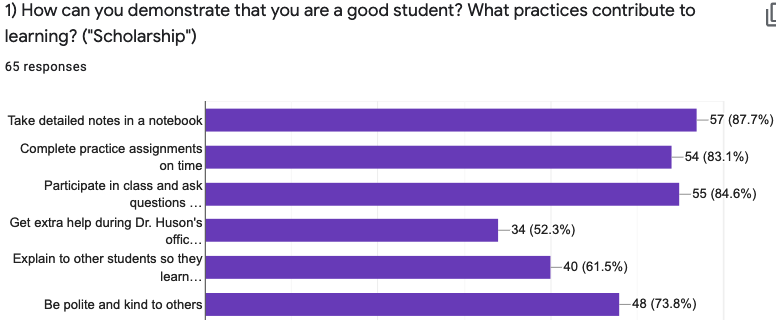
\includegraphics[width=.95\textwidth]{../graphics/scholarship-bar-chart.png}
  \begin{enumerate}
    \item Participate: Attendance (Google Classroom), Classkick
    \item Practice assignments: Khan Academy, Deltamath, 1.5 worksheet
    \item Detailed notes: Notebook treasure hunt uploads (weekend)
  \end{enumerate}
\end{frame}

\begin{frame}{What do I know, what can I do assessment}
  {1: Well below, 2: Approaching, 3: Meets expectations, 4: Exceeds}
  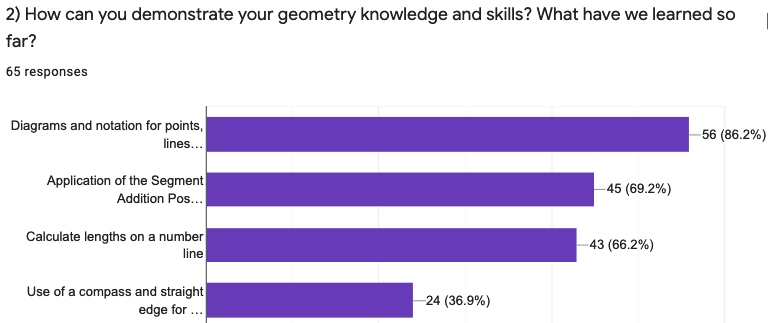
\includegraphics[width=.95\textwidth]{../graphics/know+do-bar-chart.png}
    \begin{enumerate}
      \item Classkick (open book, timed; use @beca324.org login):\\ Diagrams \& notation, segment addition, number line lengths
      \item Project: Construction of an equilateral triangle
    \end{enumerate}
  \end{frame}

\begin{frame}{Scholarship: Participation in synchronous classes}
  Participation with classmates in the lessons conducted by the teacher is one of the primary inputs to learning.\\[0.25cm]
  Among Geometry students, $84.6\%$ considered it important. \vspace{0.5cm}
    \begin{table}[ht]
      \textbf{Participation Grade}
      \begin{tabular}[t]{p{0.25\linewidth} c c c }%{|p{2.4cm}|p{5.5cm}|p{8cm}|p{4cm}|}
        \hline
        1. Well below \newline expectations & 2. Approaching & 3. Meets & 4. Exceeds \\
        \hline
        \hspace{0.5cm}$<75\%$ & 75+\% & 100\% &  \\[0.25cm]
        \multicolumn{4}{c}{based on 11 assignments in Google Classroom (no late penalty)} \\[0.25cm]
        \hline
      \end{tabular}
  \end{table} \vspace{0.25cm}
  You must also load Genuis Scan and register in \emph{Classkick} as a portfolio user, or lose one level
  \vspace{1cm}
\end{frame}

\begin{frame}{Scholarship: Practice assignments}
    ``Doing your work'' is how math skills and knowledge are gained.\\[0.25cm]
    Completing assignments on time was cited by $83.1\%$ of students. \vspace{0.5cm}
      \begin{table}[ht]
        \textbf{Practice Grade}
      \begin{tabular}[t]{p{0.25\linewidth} c c c }%{|p{2.4cm}|p{5.5cm}|p{8cm}|p{4cm}|}
        \hline
        1. Well below \newline expectations & 2. Approaching & 3. Meets & 4. Exceeds \\
        \hline
        \hspace{0.25cm} 0 or 1 out of 5 & 2 / 5 & 3 or 4 / 5 & 5/5 \\[0.25cm]
        \multicolumn{4}{c}{1.1 Khan Academy, Deltamath (3), 1.5 Worksheet} \\[0.25cm]
        \hline
      \end{tabular}
    \end{table} \vspace{0.25cm}
      Satisfactory completion of an assignment requires \emph{effort}, but not perfection. (a score of $65\%$ is usually sufficient)
      \vspace{1cm}
  \end{frame}

  \begin{frame}{Scholarship: Taking notes}
    Writing mathematics helps you learn and gives you notes to study.\\[0.25cm]
      Students said taking notes in a notebook was the most important practice for successful learning $87.7\%$. \vspace{0.5cm}
      \begin{table}[ht]
        \textbf{Notebook Grade}
        \begin{tabular}[t]{p{0.25\linewidth} p{0.25\linewidth} p{0.15\linewidth} p{0.25\linewidth}}
          \hline
          1. Well below \newline expectations & 2. Approaching & 3. Meets & 4. Exceeds \\
          \hline
          Missing several notes & Largely complete & Detailed, \newline complete & Detailed, complete, neat \& organized \\[0.25cm]
          \multicolumn{4}{c}{1.6 Notebook ``treasure hunt''} \\[0.25cm]
          \hline
        \end{tabular}
      \end{table} \vspace{0.25cm}
    Scan of pages must be uploaded (Genius app) \\one level penalty otherwise \vspace{1cm}
  \end{frame}

  \end{document}